\documentclass[12pt,a4paper,oneside]{book}

\usepackage[T1]{fontenc}
\usepackage[utf8]{inputenc}
%\usepackage[english]{babel}
\usepackage{lmodern}
\usepackage{amsmath,latexsym,amsthm,amsfonts,epsfig}
\usepackage{graphicx}
\usepackage{svg}
\usepackage{tabularx}
\usepackage{pdflscape}
\usepackage{lipsum}
\usepackage{color}
\usepackage{afterpage}
\usepackage{rotating}
\usepackage[left=3.5cm, right=2.5cm]{geometry} 
\usepackage{graphicx}
\usepackage{listings}% listing kodu
\usepackage{dcolumn}
\usepackage{fancybox}
\usepackage{float}
\usepackage{multirow}
\usepackage{longtable}
\usepackage{enumerate}
\usepackage[titletoc]{appendix}
\usepackage{fancyhdr}
\pagestyle{fancy}
\graphicspath{{./graphics/}}
\fancyhf{}
% numery stron: lewa do lewego (marginesu), prawa do prawego 
\fancyhead[LE,RO]{\textbf{\thepage}} 
% prawa pagina: zawartość \rightmark do lewego, wewnętrznego (marginesu) 
\fancyhead[LO]{\small\sffamily \nouppercase{\rightmark}}
% lewa pagina: zawartość \leftmark do prawego, wewnętrznego (marginesu) 
\fancyhead[RE]{\small\sffamily \nouppercase{\leftmark}}
% kreski oddzielające paginy (górną i dolną):
\renewcommand{\headrulewidth}{0.4pt}
\renewcommand{\footrulewidth}{0.0pt}
\newcounter{magicrownumbers}
\newcommand\rownumber{\stepcounter{magicrownumbers}\arabic{magicrownumbers}}


 \lstset{
       	breaklines=true,
			language=C,
	%		numbers=left, numberstyle=\small, stepnumber=5, numbersep=5pt,
			keywordstyle=\bfseries
    }

%\usepackage{thebibliography}
\newcommand{\n}{\textcolor{blue}} %nowododany tekst
\newcommand{\ii}{\textit}
\clubpenalty=10000 % pierwszy wiersz akapitu nie będzie kończył strony (nie używam tego ustawienia)
\tolerance = 500 \pretolerance = 900 %% skład z większą `tolerancją' (można te wartości zwiększyć bardziej)
\hbadness= 1450 %% zmniejsza liczę wyświetlanych ostrzeżeń (można zwiększyć, ale bez przesady)
%\hfuzz = 1.5pt %% tekst może sterczeć ma marginesie na 1,5pt (ok. 0,5mm)
\footskip=27pt
%\renewcommand*{\appendixtocname}{Dodatki}

\begin{document}
\titlepage{
{\bf
\begin{center}
\begin{minipage}[t]{0.55\linewidth}
\begin{center}
\mbox{}\\
Politechnika Warszawska\\
\mbox{Wydział Elektroniki i Technik Informacyjnych}\\
Instytut Informatyki\\
\end{center}
\end{minipage}
\hfill
\begin{minipage}[t]{0.4\linewidth}
\begin{flushright}
Rok akademicki 2013/2014
\end{flushright}
\end{minipage}
\vspace{1cm}
\begin{figure}[H]
\centering
%\includegraphics[width=0.21\textwidth]{pw.png}
\end{figure}
\vspace{0.5cm}
{\Large PRACA DYPLOMOWA MAGISTERSKA}
$$ \,$$
{\large Paweł Szostek}
$$ \,$$
{\LARGE Metadata extraction from scholarly publications}
\end{center}
\vfill
\begin{flushright}
\begin{minipage}[t]{0.4\linewidth}
\begin{center}
\normalsize
Opiekun pracy\\
prof. dr hab. inż. Piotr Gawrysiak\\
\end{center}                                     
\end{minipage}
\end{flushright}
$$ \,$$
$$ \,$$
\begin{flushleft}
\begin{minipage}[t]{0.45\linewidth}
\normalsize
Ocena:............................................ 
\linebreak \linebreak \linebreak
.......................................................
\begin{center}
Podpis Przewodniczącego \\
\mbox{Komisji Egzaminu Dyplomowego}
\end{center}
\end{minipage}
\end{flushleft}
}}
\pagenumbering{arabic}
\newpage
\mbox{}
\newpage
\mbox{}
%\def\contentsname{List of content}
\linespread{1.3}
\tableofcontents

\chapter{Introduction}
Digital libraries gained a lot of momentum in the recent years. The amount of publications held there is enormous and constantly growing. Collecting them in digital repositories raised many problems, where many of them go beyond acquisition issues - they have to be to be organized and classified in order to improve various retrieval procedures. Moreover, with time the purpose of the digital libraries has been evolving from a place where publications were stored, over search engines to quickly filter out publications relevant to certain topic, to frameworks used for analysis of collaboration patterns, researchers' professional network analysis, calculation of productivity and efficiency factors such as H-index (\cite{Hirsch}) or G-index or looking for emerging trends and topics in science.
All this research depends on a reliable source of full article texts and corresponding metadata, being both an input for analysis algorithms.

Even though there was a huge progress in science as such, scholarly publishing relies on methods invented more than two decades ago, which is an immense time in digital world. The most common format in digital publishing is PDF (Portable File Format), which focuses on how the document is rendered in reader's browser making it highly portable across hardware and software platforms, but without putting to much focus on metadata, which are understood here literally as \textit{data about data}. Articles are very often published and distributed in this format resulting in losing metadata. Their recovery can be performed either manually by a human worker or by a computer program. 

A modern, fully functional framework for digital libraries, in order to be useful and to provide high quality services, has to have access not only to the full texts of the articles and books that it stores, but also to their metadata. The metadata, data describing data, include such information as: document authors, document title, document abstract, keywords, document references and others. The purpose of obtaining the metadata is twofold. Firstly, they are indispensable when implementing a search engine, being an invaluable tool for all researchers looking for articles needed in their research field. Secondly, a subset of metadata, i.e. article authors and references are needed for various ranking algorithms based on citation count, such H-index \cite{Hirsch}, Impact Factor and other bibliometric indicators.

\section{Problem statement}
Regrettably, usually a digital library has to deal with the resources without any metadata provided by the publisher. In this case, the number of articles makes it barely possible to process them manually. It might also happen that the metadata available are not trustworthy or are faulty or partially missing. In these cases a digital library needs a way to obtain them automatically or semi-automatically.

This thesis presents CERMINE - a system for automatic extraction of metadata from scholarly publications, and GROTOAP2 - Ground-truth publication dataset. At its core CERMINE uses supervised machine learning algorithms, where labeled training samples from GROTOAP2 are used to train the system to recognize and assign individual elements of an article into classes depending on their function in an article. In a multi-stage process CERMINE extracts metadata, full text and bilbiographic references from an input article. The system was developed jointly by the author and his team mates as a part of work duties in Interdisciplinary Center for Mathematical and Computational Modeling at the University of Warsaw. However, their work will not be described extensively in this document and the authorship of each piece of the system will be marked explicitly. The system has been recently presented at the Force2015 meeting (\cite{Force2015}). Furthermore, an article on CERMINE was presented in the 11th IAPR International Workshop on Document Analysis Systems (\cite{DominikaTkaczykPaweSzostekMateuszFedoryszakPiotrJanDendek2014}). GROTOAP2 article was published in D-Lib magazine, volume 20. (\cite{DominikaTkaczykPaweSzostek2014}).
Information on the access to the source code and other resources is included in the appendix \ref{app:resources}.

\section{Related work}
Extracting metadata from scholarly publications is a well-studied problem. In the past, the algorithms expected scanned documents as an input and were generally formulated as image recognition problem. Those were built in the period when scholarly communication was present mainly or uniquely in a printed form and each article, before becoming available in a digital way, had to be scanned. Such approaches were presented in \cite{Thoma2001} and \cite{Flynn2007}.

Nowadays, a digital library has to cope with born-digital documents, where the letter recognition stage is omitted and processing starts with building up words and lines of text based on single characters. In the past several approaches using machine learning methods were presented.

In \cite{Esposito2008} there is presented a method for processing PostScript and PDF files using various machine learning methods in order to extract metadata.

\cite{Marinai2009} extracts basic metadata from scientific papers by, first of all, using various rules to perform segmantations of characters extracted from text and then employing a neural network to assign classes to blocks of text. Results are corrected by comparing them with an external bibliographic database.

In the approach proposed by \cite{Chen.2010} PDF files are first transformed into HTML format, then metadata is extracted using Hidden Markov Model. The authors test their approach using a set of 458 articles for VLDB conferences.

Both \cite{HuiHan} and \cite{HuiHan2005} present an approach of employing mixed Hidden Markov Model/Support Vector Machines algorithm to perform metadata and references extraction. Unlike in our approach, they do not take sequency-oriented information into considaration.

Finally, the TeamBeam algorithm, described in \cite{Kern2012}, uses a Maximum Entropy classifier to include sequence-related information in the classification. This algorithm is applied only to the first page of an article, therefore focusing only on metadata.


\chapter{Theory}
\section{Motivation}
\section{Statistical learning}
The main objective of statistical learning is to find a non-trivial description of dependencies between data gathered by measuring objects and the objects themselves. The measurement, known also as input data, is known for all of the objects under research. The property that is being looked for, on the contrary, is known uniquely for a subset of objects. The main goal of the machine learning is to figure out, in an automated way, an algorithm allowing to reason values of the properties of interest for all available input objects.

As a classical example of machine learning we might take an application in the medical diagnosis. In this case, the input data are the data obtained by performing medical analysis and medical interview. The outcome of the algorithm is a probability of patient suffering from certain disease
\section{Classification as supervised learning method}
The goal of all classification is determine to which category a new observation belongs, being given a training set consisting of samples belonging to some predefined categories. Training samples have form of n-dimensional vectors, where $n$ is the number of explanatory variables, known as well as ``features''. Features are values that express some traits of the classified elements. They can be real-numbers (e.g. 1.23, 3.14), interger-numbers (e.g. 1,2,3) or categorical values (e.g. {Circle, Square, Trapezoid}, {Large, Medium, Small}, {1,0} etc. ).

In the thoery of statistical learning, classification is considered as an example of supervised learning tasks, i.e. learning on the basis of training set for which the categories of elements are available.

% Building a classifier requires at least:
% \begin{enumerate}
% \item classification algorithm,
% \item object features,
% \item classification algorithm parameters.
% \end{enumerate} 

\section{Support Vector Machines}\label{sec:svm}
One of the most successful and broadly known techniques in machine learning are Support Vector Machines, whose theory was developped by Cortez and Vapnik. The basic idea is given a set of two classes of N-dimension points to find a hyperplane which seperates an N-dimensional space into two subspaces, so that each of them contains points belonging to only one class. Since the two classes might not always be linearly separable, SVM introduces an idea of kernel-induced space which casts the points into a higher dimensional feature space where the new points are linearly-separable. In the section \ref{subsec:linear_svm} there is a detailed description of the theoretical fundaments. In its original version the SVM classifier is a binary classifier, meaning that each point in the training sets belongs to one and only on of two classes and so the unknown points do.

CERMINE internally leverages SVM to classify its content based on the training database. This is why it is important to get acquainted with this algorithm in-depth. 

\subsection{Linearly separable Support Vector Machines} \label{subsec:linear_svm})
In the very basic example of SVM, namely a linear SVM, is to assign each new sample to one of the two classes, being given a set of learning samples. All the points, both being the learning samples and the unknown samples, are usually tuples of values of certain features.

Let us assume that we have a set of learning samples $L$, where each samples is labeled $l_i$, whereas $i$ is the index of the learning sample and $I$ is the set of these indices. Each training sample has $d$ values, so is a $d$-dimensional tuple ($x_i \in \mathbb{R}^d$) and a class label $y_i$ being on of two values ${-1, 1}$. We can sum up these assumptions with the following equation:
\begin{equation}
\forall{i \in I} \quad \left(x_i, y_i\right) : x_i \in \mathbb{R}^d, y_i \in \{-1, 1\}
\end{equation} 

For the sake of simplicity let us assume that the set of learning samples is linearly separable. We will label the separating hyperplane as $H$. Obiously, in a general case there is an infinite number of such hyper-planes what is shown on the figures \ref{fig:inf_hyperplanes} (in this case $I=5$ and $d=2$) and \ref{fig:optimal_and_suboptimal}. The two dimensions are marked as $x[0]$ and $x[1]$.

\begin{figure}[t!]
\centering
\begin{minipage}[t!]{0.45\linewidth}
 % \centering
  \includesvg[width=7cm]{graphics/hyperplanes}
  \caption{There might exist an infinite number of hyperplanes separating two groups of points. SVM's task is to find a hyperplane that maximizes distance to all data points.}
  \label{fig:inf_hyperplanes}
\end{minipage}
\quad
\begin{minipage}[t!]{0.45\linewidth}
 % \centering
  \includesvg[width=7cm]{graphics/optimal_and_suboptimal}
  \caption{There were chosen two alternative lines separating the training points. The dotted line maximizes the distance to support points, whereas the dashed one is sub-optimal.}
  \label{fig:optimal_and_suboptimal}
\end{minipage}
\end{figure}

We can describe a hyperplane $H$ with a general formula:
\begin{equation}
w \cdot x+b = 0
\end{equation}
Obviously, the number of such hyperplanes is infinite. Let us focus on a hyperplane $H$ that is equally distanced to points from both class. Let us now focus on two hyperplanes parallel to each other that separate the space. Let us label them as $H_{-1}$ and $H^{+1}$, whereas the former is stuck to a point from class $-1$ and the latter to a point belonging to class $+1$. They both maximize the distance to the objects of the other class and therefore are parallel to each other. These hyperplanes are shown on the figure \ref{fig:two_hyperplanes}.

\begin{figure}[htbp]
  \centering
  \includesvg[width=7cm]{graphics/two_hyperplanes}
  \caption{Hyperplane $H$ separates perfectly points belonging to two classes. It is equally distanced to hyperplanes $H_{-1}$ and $H_{+1}$ which are stuck to objects of classes $-1$ and $+1$ respectively.}
  \label{fig:two_hyperplanes}
\end{figure}


We can describe them with the following equations:
\begin{equation}
w^T x_i+b = 1
\end{equation}
\begin{equation}
w^T x_i+b = -1
\end{equation}
Because $H_{-1}$ and $H_{+1}$ are decision boundaries, there are no points in between them what can be summarized in the following equations:
\begin{equation} \label{eq:plus_one}
w^T x_i+b \ge 1 \quad \forall \left(x_i, y_i\right) : y_i=1
\end{equation}
\begin{equation} \label{eq:minus_one}
w^T x_i+b \le -1 \quad \forall \left(x_i, y_i\right) : y_i=-1
\end{equation}
We can unify equations \ref{eq:plus_one} and \ref{eq:minus_one} by a generalized equation:
\begin{equation}
y_i\left(w^T x_i+b\right)-1 \ge 0
\end{equation}
For each data point we might caclulate the distance to any of the hyperplanes:
\begin{equation} \label{eq:distance}
d\left(\left(w,b\right), x_i\right) = \frac{y_i\left(x_i\cdot w + b\right)}{||w||} \ge \frac{1}{||w||}
\end{equation}
To make the decision boundary most accurate, we are intuitively looking for a hyperplane that maximizes the distance to all the data points. This in turn minimizes the probability of an erronous classification of unknown data and avoids introducing a bias. According to the equation \ref{eq:distance} this can be achieved by maximizing $\frac{1}{||w||}$ or alternatively by minimizing the $||w||$ vector. We can leverage the fact that $||w||$ is a non negative value and for sake of simplicity of calculations minimize $\frac{1}{2}||w||^2$ subject to $y_i\left(w^T x_i+b\right) \ge 1 \forall i$ (note that $||w||^2=w^Tw$).

This problem will be solved with the method of Lagrange multipliers. The Langragian is calculated as follows:
\begin{equation}
\mathcal{L} = \frac{1}{2}w^Tw + \sum_{i=1}^{n}\alpha_i\left(1-y_i\left(w^Tx_i+b\right)\right)
\end{equation}
In this equation $\alpha$ is a vector of Lagrange multipliers. The problem is reduced to finding a saddle point where the function has its maximum value. Thus, by setting the Langrangian to 0 with respect to $w$ and $b$ we get:

\begin{equation}
w = \sum_{i=1}^{n}\alpha_i\left(-y_i\right)x_i=0 \Rightarrow w = \sum_{i=1}^{n}\alpha_i y_i x_i \\
\sum_{i=1}^{n}\alpha_i y_i=0
\end{equation}

If we substitute $w=\sum_{ix=1}^{n}\alpha_i y_i x_i$ in the formula for $\mathcal{L}$ we have
\begin{eqnarray*}
\mathcal{L} & = &\frac{1}{2}\sum_{i=1}^{n}\alpha_iy_ix_i^T \cdot \sum_{j=1}^{n}\alpha_jy_jx_j+\sum_{i=1}^{n}\alpha_i\left(1-y_i\left(\sum_{j=1}^{n}\alpha_jy_jx_j^Tx_i+b\right)\right) \\
& = &\frac{1}{2}\sum_{i=1}^{n}\sum_{j=1}^{n}\alpha_i\alpha_j y_i y_j x_i^T x_j + \sum_{i=1}^{n}\alpha_i-\sum_{i=1}^{n}\alpha_i y_i \sum_{j=1}^{n}\alpha_j y_j x_j^T x_i -b\sum_{i=1}^{n}\alpha_i y_i \\
& = &-\frac{1}{2}\sum_{i=1}^{n}\sum_{j=1}^{n}\alpha_i\alpha_j y_i y_j x_i^T x_j + \sum_{i=1}^{n}\alpha_i
\end{eqnarray*}

This equation can be used to define a dual problem:
\begin{eqnarray*}\label{eq:svm_dual}
max -\frac{1}{2}\sum_{i=1}^{n}\sum_{j=1}^{n}\alpha_i\alpha_j y_i y_j x_i^T x_j + \sum_{i=1}^{n}\alpha_i \\
subject to \alpha_i \ge 0, \sum_{i=1}^{n} \alpha_iy_i =0
\end{eqnarray*}

The problem above is a quadratic programming problem that always has a solution. Points $x_i$ with non-zero $\alpha_i$ are called support vectors. These are the points that determine the decision boundary.

\subsection{Non-linearly separable Support Vector Machines}
The assumption regardin linear separability of training points cannot be always met. In this section there will be presented an approach that does not require points to be linearly separable. The basic idea here is to allow misclassification, but to minimize the error on the same time. This method is known as Cost-SVM or soft margin method. In general, it allows the points to be on the ``wrong'' side of the hyperplane, but a penalty function is introduced.
Let us label with $\xi_i$ the error in classification of the $i$-th point, i.e. its distance to the classification plane in case when it is misclassified. This variable is called ``error variable'' or ``slack variable''. In addition, let us label with $C$ a tradeoff parameter between error and margin. Now, the minimized function is expressed as follows:
\begin{equation}
\frac{1}{2}||w||^2 + C \cdot \sum_{i=1}^{n}\xi_i
\end{equation}
with the following constrains:
\begin{equation}
y_i \left(w^Tx_i+b\right) \ge 1-\xi_i, \quad \xi_i>0
\end{equation}
The dual problem becomes the following:
\begin{align*}
max. & W(\alpha) = \sum_{i=1}^{n}\alpha_i-\frac{1}{2}\sum_{i=1}^{n}\sum_{j=1}^{n}\alpha_i\alpha_jy_iy_jx^T_ix_j \\
subject to & C \ge \alpha_i \ge 0, \sum_{i=1}^{n}\alpha_iy_ix_i=0
\end{align*}

\subsubsection{Nonlinear Support Vector Machines}
So far we considered only linear SVM, so these with linear decision boundary. While this solution is very simple from the computational and conceptual point of view, the results yielded by the method might be suboptimal. In this section we will present a generalized version of the algorithm, in which training points $x_i$ will be transformed to a higher dimensional space. This will allow to perform a linear division of the transformed feature space equivalent to a non-linear operation in the original space i.e. a hyper-surface instead of a hyper-plane, e.g a curve in 2-dimensional space. Example of such transformation is shown on the figure \ref{fig:2dto3d}.

\begin{figure}[htbp]
  \centering
  \includesvg[width=10cm]{graphics/2dto3d}
  \caption{An example of a transformation from a two-dimensional to a three-dimensional space. In the original space the points are clearly not linearly separable. After applying a tranformation kernel, they can be separated with a plane.}
  \label{fig:2dto3d}
\end{figure}

If we come back to the equation \ref{eq:svm_dual} we will se that the data points appear only as inner products ($x_i^Tx_j$). This means that there is need to know the mapping to the higher dimensional feature space explicitely. \\
Let us define the kernel funtion $\mathcal{K}$ as follows:
\begin{equation}
K(x_i, x_j) = \phi(x_i)^T \cdot \phi{x_j}
\end{equation}

Under certain circumstances it is feasible to obtain analytically $\phi$ being given $\mathcal{K}$. As an example let's take $\mathcal{K}(u, v) = (1+u^Tv)^2$. Then when $n=2$, i.e. $u=(u_1,u_2)$ and $v=(v_1, v_2)$ we get:
\begin{align*}
\mathcal{K}(u, v) & = & (1+u^Tv)^2 \\
& = & 1 + u_1^2v_1^2+2u_1v_1u_2v_2+u_2^2v_2^2+2u_1v_1+2u_2v_2 \\
& = & (1, u_1^2, \sqrt{2}u_1u_2, u_2^2, \sqrt{2}u_1, sqrt{2}u_2)^T(1, v_1^2, \sqrt{2}v_1v_2, v_2^2, \sqrt{2}v_1, sqrt{2}v_2) \\
& = & \phi(u)^T\phi(v)
\end{align*}
A kernel function $\mathcal{K}$ must be symmetric, continuous and have a positive definite Gramian Matrix. If the kernel function does not satisfies these conditions, then the dual problem might have no solutions.
There are three most commonly used kernel functions families: polynomial, sigmoid and radial (called also RBF).
A polynomial kernel is expressed as follows:
\begin{equation}
\mathcal{K}(x_i, x_j) = (\gamma x_i^Tx_j + c)^d \\
\end{equation}
where the parameters are:
\begin{itemize}
\item $c$ is a zero-degree term,
\item $d$ is the degree of the polynomial,
\item $\gamma$ is a generic coefficient used to parametrize the kernel.
\end{itemize}
When $d=1$ we say that a kernel is linear. This case has been described in the section \ref{subsec:linear_svm}.
\\
The most common variant of radial kernels is a gaussian distribution:
\begin{equation}
K(x_i, x_j) = e^{-\gamma|x_i-x_j|^2}
\end{equation}
where $\gamma$ is often replaced with $\frac{1}{2\sigma^2}$, so it can be interpreted as a variation around distribution's deviation.
\subsection{Feature selection and scaling}

\subsection{Model selection}
\section{Fundamentals of scholarly communication}
\subsection{Motivation behind publication analysis tools}

\chapter{System architecture}
CERMINE workflowed is composed of a multi-part pipeline, out of which every stage is treated as a separate module and can be maintained and developped independently. For implementation of the majority of non-trivial problems we used supervised and unsupervised machine learning algorithms, that gave a lot of elasticity and allow to adapt to new document layouts.

\quad
CERMINE workflow consists of the following distinguishable stages:
\begin{enumerate}
    \item \textbf{Text extraction} takes place at the very beginning of metadata extraction process. CERMINE using pdfbox, an external library for manipulating PDF content, extracts a stream of characters, together with their geometrical properties, from the input files.
    \item \textbf{Text segmentation} builds up blocks of text from a set of characters using their position and size. This stage uses Docstrum algorithm, coded by Krzysztof Rusek and described in details in \cite{O'Gorman1993}. It is therefore beyond the scope of this work and will not be mentioned hereafter.
    \item \textbf{Resolution of the reading order} aims figuring out the order in which blocks of text are meant to be read. While this task is trivial to a human reader, it is tricky to implement an elastic algorithm suitable for different article layouts.
    \item \textbf{Basic structure extraction} takes a PDF file on the input and produces a geometric hierarchical structure representing the document. The structure is composed of pages, zones, lines, words and characters. The reading order of all elements is determined. Every zone is labelled with one of four general categories: \verb+METADATA+, \verb+REFERENCES+, \verb+BODY+ and \verb+OTHER+.
    \item \textbf{Metadata extraction} part analyses parts of the geometric hierarchical structure labelled as \verb+METADATA+ and extracts a rich set of document's metadata from it.
    \item \textbf{References extraction} part analyses parts of the geometric hierarchical structure labelled as \verb+REFERENCES+ and the result is a list of document's parsed bibliographic references.
    \item \textbf{Text extraction} part analyses parts of the geometric hierarchical structure labelled as \verb+BODY+ and extracts document's body structure composed of sections, subsections and paragraphs. 
\end{enumerate}
A diagram of the above mentioned workflow can be found in the figure \ref{fig:pipeline}.
\begin{figure}[h]
  \centering
  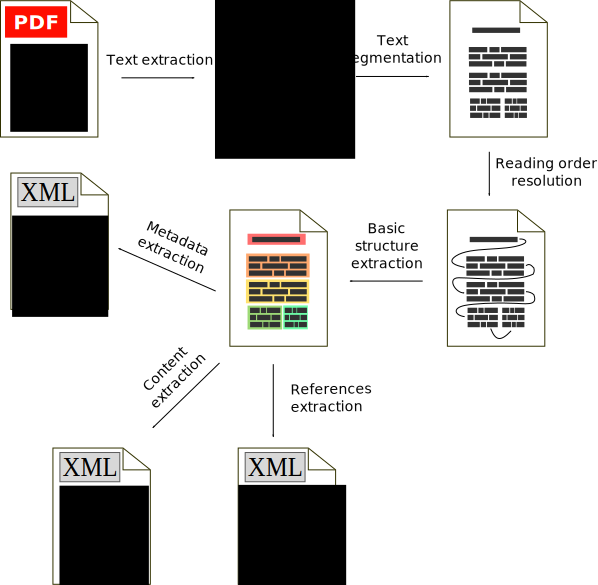
\includegraphics[width=14cm]{graphics/pipeline}
  \caption{A schematic diagram of CERMINE's workflow.}
  \label{fig:pipeline}
\end{figure}

\section{Structure extraction}
\subsection{Character extraction}\label{sec:character_extraction}
PDF document as such consists of a stream of characters, whereas position of each character in the stream doesn't have to be related, and usually is not, to its position in the text. Extraction of the characters is achieved using iText library. This part of the system was entirely implemented by Dominika Tkaczyk and will not be described in this work.
\subsection{Page segmentation}\label{sec:page_segmentation}
Page segmentation is a task of clustering a set of characters into blocks of text. Implemented system uses internally the Docstrum algorithm, described in details in \cite{O'Gorman1993}. It is a bottom-up approach based on
nearest-neighborhood clustering of connected components extracted from the document. $K$-neareast neigbours for each component are found and text lines are found based on a threshold of the angle between component centroids. Then, histograms of components spacing are used to detect inter-character distance in a word and between words. The algorithm has a set of thresholds that have to be set based on experiments with various documents. The algorithm was implemented by Krzysztof Rusek and tuned by Dominika Tkaczyk and therefore will not be described in this document in details.

\subsection{Reading order resolving}\label{sec:reading_order}
Resolution of Reading Order is a process aiming to transform text zones from a two-dimensional space (as they are laid out on the paper) to a single-dimensional space, i.e. as they are read by a human. Usually this is done by going from left to right and from top to bottom, but there are a lot of cases that made this na\"\i ve approach less efficient. This includes multi-column layout, page numbers, textual elements of figures, figures' and equations' labels.
\qquad
As already described in \cite{DominikaTkaczykPaweSzostekMateuszFedoryszakPiotrJanDendek2014}, a PDF file contains a stream of characters that undergoes processes of extraction and segmentation. This results in a list of pages consisting of zones, lines, words and chunks of text. These elements need to be put together in the same order as that would be done by a human reader.\\
To this end, a bottom-up strategy is applied: firstly characters are sorted within words and words within lines in ascending order according to X coordinate value. Afterwards, lines are sorted with Y coordinate as the key. As next we need to figure out zones' order. Below we describe a heuristic responsible for setting order of text zones Its fundamental principle was taken from \cite{ROR_source}. A schematic diagram of this phase can be found in the figure \ref{fig:reading_order}.
\begin{figure}[]
  \centering
  \includesvg[width=12cm]{graphics/ro}
  \caption{A schematic diagram of reading order resolving. Firstly, distances between text zones are calculated. Then, zones are hierarchicaly grouped according to distances between them. Finally, the tree is in-order traversed and a list of zones in created.}
  \label{fig:reading_order}
\end{figure}
\begin{enumerate}
\item For each pair of items inside a single page boundaries a free space between them is calculated. On the figure \ref{fig:reading_order} this space is ilustrated as the black area between two zones. The full implementation of the algorithm is included in the appendix \ref{appendix:ror}. Below is a detailed description of the steps taken.
	\begin{enumerate} 
	\item Formally the free space $S$ can be expressed as $S = A_d - (A_1+A_2)$, where $A_1$ and $A_2$ are areas of the two zones and $A_d$ is area of the smallest rectangle in which two objects can fit. This rectangle has to have sides parallel to the X and Y axes.
	\item To include preference for vertical clustering (and to avoid joining blocks horizontally when multi-column layouts are present) a cosine of the angle $\alpha$ between the vector $\vec{v}$ connecting two objects' geometrical centers and vector $\vec{x}$ being a projection of the vector $\vec{v}$ on the X axis is calculated. This was illustrated in the figure \ref{fig:angle_alpha}. The formula $\cos\alpha = \frac{\vec{v} \cdot \vec{x}}{|\vec{v}||\vec{x}|}$ is employed.
	\item Free space $S$ is multiplied by sum of coefficient $M$ and $\cos\alpha$. Coefficient $M$ is introduced in order to prevent situations when more than two zones have the same width and lay in-line with respect to the Y axes. Then, for each of them the calculated distance would be equal to zero. In such cases we prefer to join these two groups between which the Euclidean distance is minimized.
	\end{enumerate}
\item A list $L$ containing triples ($O_1$, $O_2$, $D$) is created (where $O_1$ and $O_2$ are zones on the page and $D$ is the distance between zones) Initially there are $\binom{N}{2}$ elements in the list.
\item List $L$ is sorted in ascending order with respect to the distance $D$. 
\item Until this list is empty, the first triple is picked (i.e. with the smallest distance $D$) and two associated objects, $O_1$ and $O_2$, are merged.
\item For each element $E$ in the $L$ recalculate the distance $D$ to the new group iff the $E$ contains $O_1$ or $O_2$ (i.e. is in form of ($O_1$, $X$, $D$) or ($O_2$, $X$, $D$)).  Insert into the list a new triple ($O_1O_2$, $X$, $D$) where $O_1O_2$ is the new group.
\item Sort the list $L$ in ascending order.
\end{enumerate}
\begin{figure}[h!]
  \centering
  \includesvg[width=8cm]{graphics/angle_alpha}
  \caption{To include preference for vertical clustering a cosine of the angle $\alpha$ between the vector $\vec{v}$ and vector $\vec{x}$ is calculated.}
  \label{fig:angle_alpha}
\end{figure}
\begin{lstlisting}[caption=Listing of the function measuring distance between two zones or zone groups.]

private double distance(BxObject obj1, BxObject obj2) {

    double x0 = Math.min(obj1.getX(), obj2.getX());
    double y0 = Math.min(obj1.getY(), obj2.getY());
    double x1 = Math.max(obj1.getX() + obj1.getWidth(),
            obj2.getX() + obj2.getWidth());
    double y1 = Math.max(obj1.getY() + obj1.getHeight(),
            obj2.getY() + obj2.getHeight());
    double dist = ((x1 - x0) * (y1 - y0) - obj1.getArea() - obj2.getArea());

    double obj1CenterX = obj1.getX();
    double obj1CenterY = obj1.getY() + obj1.getHeight() / 2;
    double obj2CenterX = obj2.getX();
    double obj2CenterY = obj2.getY() + obj2.getHeight() / 2;

    double obj1obj2VectorCosineAbs = Math.abs((obj2CenterX - obj1CenterX) / Math.sqrt((obj2CenterX - obj1CenterX) * (obj2CenterX - obj1CenterX) + (obj2CenterY - obj1CenterY) * (obj2CenterY - obj1CenterY)));
    final double M_COEFF = 0.5;
    return dist * (M_COEFF + obj1obj2VectorCosineAbs);
}
\end{lstlisting}
\section{Initial zone classification}
After the stages described in sections \ref{sec:character_extraction}, \ref{sec:page_segmentation} and \ref{sec:reading_order} the document can undergo the two phases of classification. Firstly, all the zones are classified to one of the four general classes: \verb+METADATA+, \verb+REFERENCES+, \verb+BODY+ and \verb+OTHER+. After this stage, more specific classifiers and algorithms can perform finer-grained analysis on the zones falling into each class. Semantics of these classes is as following
\begin{itemize}
\item \verb+METADATA+ contains all the data which do not constitute the proper content. This includes publication elements such as: title, author name, affiliation, bibliographic informations, abstract etc.
\item \verb+BODY+ contains text of the publication. This includes the chapters, figures, tables, equations, plots, acknowledgments, headings, contribution statements, conflict statements and attachments.
\item \verb+REFERENCES+ contains article's references,
\item \verb+OTHER+ contains misclassified zones and page numbers. It is a result of a non-ideal dataset, being tagged only to some extent. When training the classifier, those unclassified zones are labeled as \verb+OTHER+. This in turn introduces some kind on additional noise. We decided that it is better to exclude a handful of zones from the further processing and classify them as \verb+OTHER+, rather than to classify them incorrectly to one of the remaining classes. Employed dataset contains 3.6\% of unknown labels, therefore we might expect a similar number of zones classified to \verb+OTHER+ in the classifier's output.
\end{itemize}
\quad
Initial classification uses Support Vector Machines as classication algorithm, with the parameters given in the table \ref{tab:initial_classifier_parameters}. A way to obtain these parameters is described in \ref{sec:svm_optimization}.
\begin{table*}
\centering
\begin{tabular}{@{}rrr@{}}
\toprule
& initial & metadata \\
\midrule
SVM type & C\_SVC & C\_SVC \\ 
kernel type & polynomial & polynomial \\
$\gamma$ & $\frac{1}{8}$ & $\frac{1}{8}$ \\ 
$C$ & 8 & 8 \\
$coef_0$ & 0.5 & 0.5 \\
$degree$ & 3 & 3 \\
\bottomrule
\end{tabular}
\caption{Parameters used in the final training of the initial classifier}
\label{tab:initial_classifier_parameters}
\end{table*} 
\section{Metadata classification}
Once the initial coarse-grained classification is done, we employ a second classifier which is specialized in classifying metadata, i.e. those zones, which initially got the \verb+METADATA+ label. This class consists of 19 labels:
\begin{itemize}
    \item \textbf{abstract} - document's abstract, usually one or more zones placed in the first page of the document;
    \item \textbf{acknowledgments} - sections containing information about document's acknowledgments or funding;
    \item \textbf{affiliation} - authors' affiliations sections, which sometimes contain contact information (emails, addresses) as well;
    \item \textbf{author} - a list of document's authors,
    \item \textbf{bib\_info} - zones containing all kinds of bibliographic information, such as journal/publisher name, volume, issue, DOI, etc.; often includes pages' headers or footers; headers and footers containing document's title or author names are also labelled as bib\_info;
    \item \textbf{body\_content} - the text content of the document, contains paragraphs and section titles;
    \item \textbf{conflict\_statement} - conflict statement declarations;
    \item \textbf{copyright} - copyright or license-related sections;
    \item \textbf{correspondence} - the authors' contact information, such as emails or addresses;
    \item \textbf{dates} -important dates related to the document, such as received, revised, accepted or published dates;
    \item \textbf{editor} - the names of the document's editors;
    \item \textbf{equation} - equations placed in the document;
    \item \textbf{figure} - zones containing figures' captions and other text fragments belonging to figures;
    \item \textbf{glossary} - important terms and abbreviations used in the document;
    \item \textbf{keywords} - keywords listed in the document;
    \item \textbf{page} number -zones containing the numbers of pages;
    \item \textbf{table} - the text content of tables and table captions;
    \item \textbf{title} - the document's title;
    \item \textbf{title\_author} - zones containing both document's title and the list of authors;
    \item \textbf{type} -the type of the document, usually mentioned on the first page near the title, such as ``research paper'', ``case study'' or ``editorial'';
    \item \textbf{unknown} - used for all the zones that do not fall in any of the above categories.
\end{itemize}
\begin{table*}
\centering
\begin{tabular}{@{}rrr@{}}
\toprule
& initial & metadata \\
\midrule
SVM type & C\_SVC & C\_SVC \\ 
kernel type & polynomial & polynomial \\
$\gamma$ & $\frac{1}{8}$ & $\frac{1}{8}$ \\ 
$C$ & 8 & 8 \\
$coef_0$ & 0.5 & 0.5 \\
$degree$ & 3 & 3 \\
\bottomrule
\end{tabular}
\caption{Parameters used in the final training of the metadata classifier}
\label{tab:metadata_classifier_parameters}
\end{table*} 


\section{Optimization of classifiers' parameters}
\label{sec:svm_optimization}
As already described in section \ref{sec:svm} CERMINE uses internally the SVM algorithm to classify  
\section{References extraction}
Reference extraction path is responisble for processing zones that were labelled as \verb+REFERENCE+ during the inital classification; it's purpose is to extract bibligraphic references together with their metadata.

To this end, the blocks of text are divided into strings containing one bibliographic reference each. This phase employs unsupervised learning whose task is to cluster all lines of references into two group - one group containing only first lines of references and the second group containing other lines. The clustering algorithm uses 5 features based on the text layout.

Afterwards, inidividual references are parsed and corresponding bibliographical data are yield back. This algorithm is based on Conditional Random Fields, thus a supervised learnign algorithm, and is implemented on the top of GRMM and Mallet packages.

Reference extraction was implemented by Mateusz Fedoryszak and is described in details in \ref{DominikaTkaczykPaweSzostekMateuszFedoryszakPiotrJanDendek2014}.
\section{Text extraction}
\section{Feature selection}
In both stages of classification we employed a set of features including almost one hundred elements. In appendix \ref{appendix:features} there is a detailed description of how their values are calculated. Briefly, they can be divided into following groups:
\subsubsection{Sequence features}
This group contains only two features: \textit{PreviousZoneFeature} and \textit{LastButOneZoneFeature}. It leverages the fact that the zones are classified after the process of reading order resolution is done. The features contain numerical value of two previous labels. In turn, this allows to incorporate sequence information into classification, which is not done in SVM by design (as opposed to for instance Hidden Markov Model).
\subsubsection{Formatting features}
This group of features contains information about graphical properties of text. It can be very helpful while certain elements in scholarly publications are usually typed with bigger font size
\subsubsection{Layout features}
These features encode information about graphical layout on the page. This includes properties of the zone itself (e.g. \textit{WidthFeature}, \textit{HeightFeature}, \textit{LineMeanWidthFeature}) as well as features of the area between text zones (e.g. \textit{HorizontalRelativeProminenceFeature},\textit{VerticalRelativeProminenceFeature}, \textit{IsHighestOnThePage}, \textit{IsGreatestOnThePage}, \textit{DistanceFromNearestNeighbourFeature}). 
\subsubsection{Semantic features}
This group of features encodes appearence of certain key-words that very often characterize certain parts of articles written with scientific english, e.g. ``keywords'', ``terms'', ``distributed'', ``reproduction'', ``open'', ``commons'', ``license'', ``creative'', ``copyright'', ``cited'', ``distribution'', ``access'', ``references'', ``author'', ``bibliography'', ``figure'', ``table'', ``editor'', ``email'', ``correspondence'', ``address'', ``abstract'', ``author details'', ``university'', ``department'', ``school'', ``institute'', ``affiliation'', ``affiliation'', ``research article'', ``review article'', ``editorial'', ``review'', ``debate'', ``case report'', ``research'', ``original research'', ``methodology'', ``clinical study'', ``commentary'', ``article'', 
 ``hypothesis'', .
\subsubsection{Special features}
This group contains features that do not fit other groups described above. This includes e.g. \textit{IsAnywhereElseFeature}, \text{BracketCountFeature}, \text{CharCountFeature}, \text{CommaCountFeature}.

\section{Learning process}
\subsection{Model cross-validation}
\chapter{Dataset}
\section{Motivation}
Despite a strong need of performing automated analyses of scholarly publications, there are not big and reliable datasets of annotated publications available publicly. Such a dataset would greatly facilitate the process of building a classifier to perform the processes automatically.
\subsection{Open Access publications}
\section{Pubmed database}
Pubmed \cite{Pubmed} is a collection of more than 24 millions articles from MEDLINE, life science journals and online books maintained by the US National Library of Medicine. This collection is digitized which means that the articles are stored in form of PDF files and can serve as a source of full texts without a need for performing Optical Character Recognition. 
The PMC Open Access Subset (abbreviated to PMC-OAS) is a part of the collection of Pubmed central available publicly with any fees. These articles are kept protected by copyrights, but can be used under the Creative Commons license that allows for more liberal usage of the resources. For the time of creating this report (June 2014) there were more than 400'000 articles available.
\section{Dataset creation}
With very limited budget it is clearly impossible to create a rich set of annotated articles by human means. Such was made in ICM in \cite{DominikaTkaczykArturCzeczkoKrzysztofRusekLukaszBolikowski2012}. GROTOAP (``GROund Truth for Open Access Publications'') created there is a collection of 113 articles in digitial form with corresponding ground-truth files. The ground truth files were tagged manualy, so precision and accuracy are guaranteed. Unluckily, these articles cover not more than 15 different layouts, which is certainly not enough when aiming to a tool applicable to the whole spectrum of publishers and layouts. This is why it was decided to create a dataset, called GROTOAP2, that could serve as a base for classifiers.
\section{The methodology of creating GROTOAP2}
As stated above, it was assumed that GROTOAP2 has to be based on open access articles. Pubmed was chosen as source of input data, as a great majority of contained articles is associated with extracted metadata. Sometimes their quality might be put in doubt, but the process was designed to automatically filter them out.
\qquad
Each article in the Pubmed dataset cames as a tarball containing the article itself (in PDF format), a metadata file (in XML) and possible some resource files, mainly including pictures extracted from the PDF. A sample content of a metadata XML is showed in the figure \ref{fig:pmc_xml}.
The general strategy for creting ground-truth files out of the PMC-OAS was to match content of the metadata files to blocks of text extracted and segmented from the provided PDF files resulting in a tagged TrueViz file. PMC-AOS metadata files are not perfect, though. There are many situations, listed below, that one has to account for. Full understanding of their structure was achieved by thorough and laborious manual analysis of many randomly picked sample files.
\begin{itemize}
\item structure of the documents varies between documents,
\item random fields might be missing or be incomplete,
\item same content (e.g. article's title) might be located under different paths, e.g. contributor's e-mail address might be found under \verb+/article/front/article-meta/contrib-group/contrib/email+ or \verb+/article/front/article-meta/contrib-group/contrib/address/email+.
\item same content might have different level of granularity, e.g. editor's name might be given as a flat string, whereas author's name might be divided into surname and given names,
\item elements of the same kind be found under different parents, e.g. figures might be located in \verb+/article/floats-wrap//fig+, \verb+/article/floats-group//fig+, \verb+/article/back//fig+, \verb+/article/body//fig+, \verb+/article/back/app-group//fig+

\end{itemize}

We use xpath to extract text entries from predefined paths. These paths are common for the documents in the Pubmed dataset. Each path is mapped to a label in our labeling system. The task consists in finding a mapping betwen NLM entries and PDF zones, so that each zone could obtain a label dependent on its path in the NLM file.

For each pair of kind (pdf\_zone, nlm\_entry) Smith-Waterman distance
is calculated (457-480) For each zone a couple of different approaches are followed in order to assign a correct label:
\begin{enumerate}
\item Take NLM entry with the highest ratio of SW distance to the number of tokens ($\frac{t1.alignment}{t1.entryTokens.size()}$). If both PDF zone and NLM entry are not empty and their size in tokens is comparable (ratio not smaller than 0.7) and length of the common substring constitutes (swLabelSim.get(zoneIdx).get(0).alignment / entryTokens.size() > 0.7) more than 70\% of the NLM entry, then assign corresponding label (483-516)
\item if the previous approach failed, take the entry with the highest SW distance. If the length of the common substring is bigger than 50\% of the number of tokens in the PDF zone (swLabelSim.get(zoneIdx).get(0).alignment / zoneTokens.size() > 0.5), then assign corresponding label, (517-540)
\item if the previous aproaches failed, a ``cumulated'' distance is calculated. This makes it possible to assign a label to these zones that form together one NLM entry, but were segmented into several parts. This applies mostly to BODY zones. For each and each entry and each zone (SW\_distance / Math.max(zoneTokens.size(), trio.entryTokens.size())) is calculated. For each zone these values are aggregated by summing them up. From all the cumulated distance the biggest one is taken. If it is greater than 0.5, the corresponding label is assigned. (542-570)
\end{enumerate}
\section{Filtering}
\include{results}
\begin{appendices}
%\appendixpage
\noappendicestocpagenum
\addappheadtotoc

\chapter{Description of classification features}
\label{appendix:features}
\newgeometry{left=2cm,right=2cm}
%\begin{landscape}

\begin{longtable}[t!]{l|l|p{9cm}}
\hline
\# & \textbf{Feature Name} & \textbf{Description} \\ \hline
\rownumber & AffiliationFeature & Tells if the zone contains one of the \{``author details'', ``university'', ``department'', ``school'', ``institute'', ``affiliation''\}\\ \hline
\rownumber & AuthorFeature & Tells if a text zone contains a word starting with ``author''\\ \hline
\rownumber & BibinfoFeature & Number of occurences of \{``cite'', ``pages'', ``article'', ``volume'', ``publishing'', ``journal'', ``doi'', ``cite this article'', ``citation'', ``issue'', ``issn''\} \\ \hline
\rownumber & BracketRelativeCount & Ratio of the number of brackets to the number of all characters \\ \hline
\rownumber & BracketedLineRelativeCount & Ratio of number of lines starting with a bracket to the number of all lines\\ \hline
\rownumber & CharCountFeature & Counts number of characters in a zone\\ \hline
\rownumber & CharCountRelativeFeature & Ratio of number of characters in a zone to the number of character on its page\\ \hline
\rownumber & CommaCountFeature & Counts number of commas in a zone\\ \hline
\rownumber & CommaRelativeCountFeature & Ratio of commas to all characters in a zone \\ \hline
\rownumber & ContainsPageNumberFeature & Tells consists of a number or is like ``Page \%d'' or ``page \%d'', where \%d is a number \\ \hline
\rownumber & CuePhrasesRelativeCountFeature & Ratio of cue phrases from \{``although'', ``therefore'', ``therein'', ``hereby'', ``nevertheless'', ``to this end'', ``however'', ``moreover'', ``nonetheles''\} to all words\\ \hline
\rownumber & DateFeature & Tells if the zone contains a string being a date with months expressed as text or as a number, with either European or American order\\ \hline
\rownumber & DigitCountFeature & Number of digits is in the zone\\ \hline
\rownumber & DigitRelativeCountFeature & Ratio of digits to all characters in the zone \\ \hline
\rownumber & DistanceFromNearestNeighbourFeature & Distance to the nearest neighbour zone or returns Double.MAX\_VALUE if there is no other zone on the page\\ \hline
\rownumber & DotCountFeature & Counts number of dots (``.'') in the zone\\ \hline
\rownumber & DotRelativeCountFeature & Ratio of number of dots to all characters in the zone \\ \hline
\rownumber & EmailFeature & Tells if the zone contains a valid e-mail address\\ \hline
\rownumber & EmptySpaceRelativeFeature & Calculates a ratio of the surface taken by the characters' bounding boxes to the area of the zone \\ \hline
\rownumber & FontHeightMeanFeature & Calculates average font size in the zone \\ \hline
\rownumber & FreeSpaceWithinZoneFeature & Difference between zone's area and total area taken by the characters\\ \hline
\rownumber & HeightFeature & Height of a zone\\ \hline
\rownumber & HeightRelativeFeature & Ratio of zone's height to the page's height\\ \hline
\rownumber & HorizontalRelativeProminenceFeature & Area taken by the zone and free area to the West and East of the page. This features tries to fit into the page a bounding box of the same height as the zone and sticking either to neighbour zones or to the page boundaries in E and W\\ \hline
\rownumber & IsAnywhereElseFeature & Tells if this zone is duplicated anywhere in the investigated document \\ \hline
\rownumber & IsFirstPageFeature & Tells if the zone is located on the first page of the document \\ \hline
\rownumber & IsFontBiggerThanNeighboursFeature & Tells whether the font of the zone is bigger than in neighbour zones\\ \hline
\rownumber & IsGreatestFontOnPageFeature & Tells if the zone has the greatest font on the page \\ \hline
\rownumber & IsHighestOnThePageFeature & Tells if the zone is the highest on the page \\ \hline
\rownumber & IsItemizeFeature & Tells if the zone contains any kind of indexing charactersic for section or enumeration numbering \\ \hline
\rownumber & IsWidestOnThePageFeature & Tells if the zone is the widest on the page\\ \hline
\rownumber & IsLastButOnePageFeature & Tells if the zone is located on the last but one page\\ \hline
\rownumber & IsLastPageFeature & Tells if the zone is located on the last page\\ \hline
\rownumber & IsLeftFeature & Tells if the zone is in the left part of the page\\ \hline
\rownumber & IsLongestOnThePageFeature & Tells if the zone contains maximal number of characters among all the zones in the page\\ \hline
\rownumber & IsLowestOnThePageFeature & Tells if the zone is most southern on the page (southern bounding box border is taken into account) \\ \hline
\rownumber & IsOnSurroundingPagesFeature & Tells if the same zone is on the previous or on the next page \\ \hline
\rownumber & IsPageNumberFeature & Tells if a zone is entirely a number \\ \hline
\rownumber & IsRightFeature & Tells if a zone is on the east side of the page\\ \hline
\rownumber & IsSingleWordFeature & Tells if a zone is one word \\ \hline
\rownumber & LastButOneZoneFeature & Tells if the zone is last but one wrt. to the reading order \\ \hline
\rownumber & LineCountFeature & Number of lines in the zone\\ \hline
\rownumber & LineRelativeCountFeature & Ratio of lines in the to all lines on the page\\ \hline
\rownumber & LineHeightMeanFeature & Mean height of the zone\\ \hline
\rownumber & LineWidthMeanFeature & Mean width of the zone's lines\\ \hline
\rownumber & LineXPositionMeanFeature & Mean distance of zone's lines to the zone's bounding box \\ \hline
\rownumber & LineXPositionDiffFeature & The feature looks at the left border of all lines within a zone and finds the most-eastern and most-western among them. A positive difference between these two values is returned\\ \hline
\rownumber & LineXWidthPositionDiffFeature & Difference between mean value of lines' left border X coordinate and zone's  \\ \hline
\rownumber & LetterCountFeature & Number of letters in the zone\\ \hline
\rownumber & LetterRelativeCountFeature & Ratio of letters in the zone to all letters on the page\\ \hline
\rownumber & LowercaseCountFeature & Number of letters in lower case in the zone\\ \hline
\rownumber & LowercaseRelativeCountFeature & Number of letters in lower case in the zone\\ \hline
\rownumber & PageNumberFeature & Page number wrt. the reading order \\ \hline
\rownumber & PreviousZoneFeature & Value of label assigned to the previous zone wrt. the reading order\\ \hline
\rownumber & ProportionsFeature & Width to height ratio\\ \hline
\rownumber & PunctuationRelativeCountFeature & Ratio of punctuation marks to all characters in the zone\\ \hline
\rownumber & ReferencesFeature & Number of characteristic enumeration indices in the zone, e.g. ``1.''.\\ \hline
\rownumber & StartsWithDigitFeature & Tells if the zone's first character is a digit\\ \hline
\rownumber & UppercaseCountFeature & Number of upper case characters in the zone \\ \hline
\rownumber & UppercaseRelativeCountFeature & Ratio of upper case letters to all characters\\ \hline
\rownumber & UppercaseWordCountFeature & Number of words starting with upper case\\ \hline
\rownumber & UppercaseWordRelativeCountFeature & Ratio of upper case words to all words\\ \hline
\rownumber & VerticalProminenceFeature & Space taken by the zone and free area to the North and South of the page. This features tries to fit into the page a bounding box of the same height as the zone and sticking either to neighbour zones or to the page boundaries in N and S \\ \hline
\rownumber & WidthFeature & Width of the bounding box in pixels\\ \hline
\rownumber & WordCountFeature & Number of words in the zone\\ \hline
\rownumber & WordCountRelativeFeature & Ratio of number of words in the zone to all words in the page\\ \hline
\rownumber & WordWidthMeanFeature & Mean width of words in the zone expressed as pixels\\ \hline
\rownumber & WordLengthMeanFeature & Mean width of words in the zone expressed as number of characters\\ \hline
\rownumber & WordLengthMedianFeature & Median of number of characters in all words \\ \hline
\rownumber & WhitespaceCountFeature & Number of white characters in the text\\ \hline
\rownumber & WhitespaceRelativeCountLogFeature & Feature calculated as $-log \frac{S}{L}$ where $S$ is zone's empty area and $L$ is zone's text length \\ \hline
\rownumber & WidthRelativeFeature & Ratio of zone's width to page's width\\ \hline
\rownumber & XPositionFeature & X coordinate\\ \hline
\rownumber & XPositionRelativeFeature & Ratio of zone's X coordinate to page's width \\ \hline
\rownumber & YPositionFeature & Y coordinate \\ \hline
\rownumber & YPositionRelativeFeature & Ratio of zone's Y coordinate to page's height \\ \hline
\end{longtable}
\restoregeometry
\setcounter{magicrownumbers}{0}
\end{appendices}
%\addtocontents{toc}{\protect\vspace{1em}\noindent{\bf Bibliografia}\hspace*{\fill}{\bf \pageref{literatura}}}
\pagebreak
\bibliography{bibliography}{}
\bibliographystyle{plain}
\end{document}

